\newpage
\section{Обслуживание пациентов}

\subsection {Регистрация обращений} \label{pol_obr}

Каждый раз при обращении пациента в ЛПУ за амбулаторной помощью, в картотеке пациентов для него регистрируется новое обращение. Обращение содержит цель, установленные диагнозы пациента, результаты осмотров и обследований, информацию о назначенных мероприятиях и их выполнении, результат обращения. На основании обращения можно распечатать <<Талон амбулаторного пациента>> (Ф. 025\slash У-12).

Для регистрации обращения на основе предварительной записи следует найти данные пациента в БД (см. п. \ref{cl_find}) и щелкнуть по соответствующей записи левой кнопкой мыши. В появившемся всплывающем окне (Рисунок \ref{img_cl_contrwin}) нужно нажать кнопку 
\includegraphics[scale=0.6]{addg}, справа от соответствующей записи на вкладке \dm{Предварительная запись}. Будет открыта страница \dm{Создание обращения}.

Кнопки \btn{Создать обращение} или 
\includegraphics[scale=0.6]{addb} позволяют создавать обращение без предварительной записи. Кнопки доступны:
\begin{itemize}
 \item Из высплывающего окна картотеки пациентов (Рисунок \ref{img_cl_contrwin});
 \item Со страницы создания и редактирования регистрационной карточки пациента. 
\end{itemize}

Дле регистрации обращения без предварительной записи нужно нажать кнопку \btn{Создать обращение} или кнопку 
\includegraphics[scale=0.6]{addb}. Если на момент регистрации обращения у пациента имеются действующие предварительные записи к другим специалистам, то появится предупреждение во всплывающем окне <<У пациента есть предварительные записи>>.Необходимо убедиться, что предварительные записи были зарегистрированы к другому врачу и только после этого продолжить регистрацию текущего обращения нажатием кнопки \btn{Все равно продолжить}. Отменить создание обращения без предварительной записи можно, нажав кнопку  \btn{Отмена} во всплывающем окне.

После подтверждения будет открыта страница \dm{Создание обращения}. На этой странице, прежде всего, необходимо убедиться, что обращение создано для нужного пациента, проверив его данные в правой верхней части окна. После этого нужно заполнить пустые и изменить неверно заполненные поля в блоке \dm{Основная информация}. Часть полей может быть заполнена на основе данных предварительной записи (если обращение создавалось на основе нее) или значениями по умолчанию.

\begin{vnim}
 Поля \dm{Дата выполнения} и \dm{Время выполнения} на данном этапе заполнять не нужно!
\end{vnim}

Все поля, кроме полей \dm{Дата выполнения} и \dm{Время выполнения} являются обязательными для заполнения.
\begin{itemize}
 \item \dm{Тип обращения} выбирается из списка значение <<Поликлиника>>.
 \item \dm{Источник финансирования} – канал оплаты обращения, выбирается из списка.
 \item \dm{Договор} – номер договора об оплате выбирается из списка. Состав списка зависит от выбранного источника финансирования.
 \item \dm{Тип события} – выбирается из списка. Состав списка изменяется в зависимости от выбранного типа обращения и источника финансирования.
 \item \dm{Лечащий врач} – врач, к которому направляется пациент в поликлинике.
 \item \dm{Подразделение} – отделение поликлиники, куда направляется пациент.
 \item \dm{Дата начала} – по умолчанию устанавливается дата предварительной записи либо текущая дата. При необходимости дату можно изменить.
 \item \dm{Время начала} – по умолчанию устанавливается время предварительной записи либо текущее время. При необходимости время можно изменить.
 \item \dm{Дата выполнения} – дата завершения обслуживания по данному обращению. Должна заполняться врачом.
 \item \dm{Время выполнения} – время закрытия обращения. Должно заполняться врачом.
\end{itemize}

После того как все поля заполнены верно, нужно нажать кнопку \btn{Создать} в правом нижнем углу страницы. Будет осуществлен переход к следующему этапу оформления обращения. Как правило, работа регистратуры ограничивается первым этапом. Последующее заполнение обращения выполняется врачом.

Если была предпринята попытка создания обращения не для того пациента или создание обращения вообще не требуется, следует нажать кнопку \btn{Отменить}. Обращение создано не будет.

\subsubsection{Регистрация платных обращений}

Если в качестве источника финансирования обращения выбрано <<Платные услуги>>, то необходимо на странице обращения зарегистрировать данные о плательщике (Рисунок \ref{img_pol_payer}). Рекомендуется сделать это при создании обращения. Однако, можно ввести эти данные и позднее, открыв обращение на редактирование. 

\begin{figure}[ht]\centering
	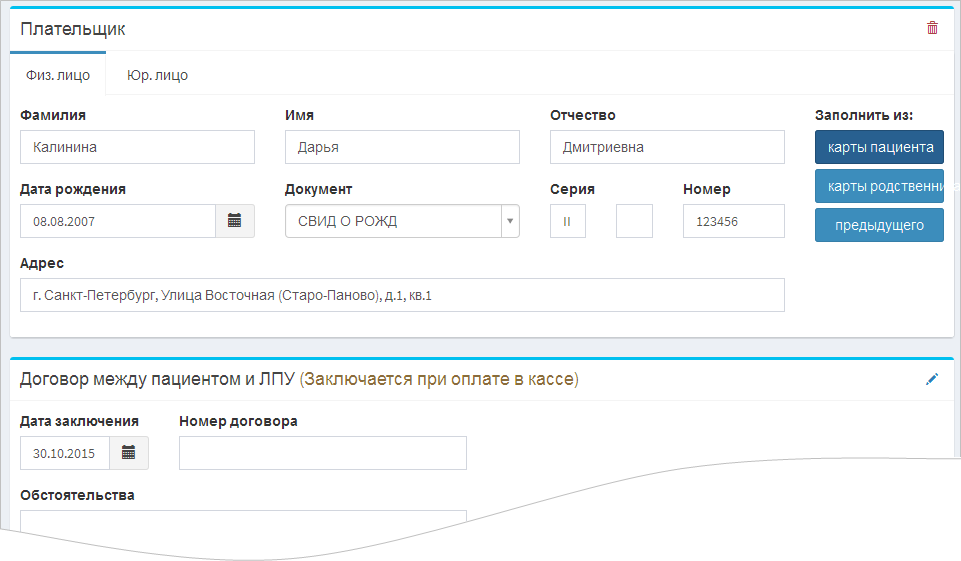
\includegraphics[width = 1\textwidth ,keepaspectratio]{pol_payer}
	\caption{Данные плательщика в обращении}
	\label{img_pol_payer}
\end{figure}

В качестве плательщика может выступать физическое или юридическое лицо.

Если плательщиком является физическое лицо, то необходимо заполнить следующие поля в подразделе \dm{Плательщик} на вкладке \dm{Физ.лицо}:
\begin{itemize}
	\item \dm{Фамилия} -- фамилия плательщика;
	\item \dm{Имя} -- имя плательщика;
	\item \dm{Отчество} -- отчество плательщика;
	\item \dm{Дата рождения} -- дата рождения плательщика;
	\item \dm{Документ} -- тип документа, удостоверяющего личность плательщика. Выбирается из раскрывающегося списка;
	\item \dm{Серия} -- серия документа, удостоверяющего личность плательщика. Серия может быть разбита на 2 отдельных поля;
	\item \dm{Номер} -- номер документа, удостоверяющего личность плательщика. 
	\item \dm{Серия} -- серия документа, удостоверяющего личность плательщика;
	\item \dm{Адрес} -- адрес регистрации плательщика, записывается в виде текстовой строки. 
\end{itemize}

Кнопки, расположенные справа от полей подраздела \dm{Плательщик}, позволяют в некоторых случаях автоматизировать заполнение данных полей. 
\begin{itemize}
	\item Кнопка \btn{карты пациента} позволяет скопировать в поля подраздела \dm{Плательщик} на вкладке \dm{Физ.лицо} данные пациента. Данную кнопку можно применять, если сам пациент является плательщиком.
	\item Кнопка \btn{карты родственника} позволяет скопировать в поля подраздела \dm{Плательщик} на вкладке \dm{Физ.лицо} данные одного из родственников пациента. При нажатии на данную кнопку появляется всплывающее окно, где необходимо выбрать одного из родственноков пациента и нажать кнопку \btn{Выбрать}. Для использования данного способа необходимо, чтобы родственник пациента был зарегистрирован в разделе \dm{Связи} регистрационной карточки текущего пациента.
	\item Кнопка \dm{предыдущего} позволяет скопировать данные плательщика из предыдущего обращения пациента (если такое имеется).
\end{itemize} 

Если плательщиком является юридическое лицо, то необходимо перейти на вкладку \dm{Юр.лицо} в подразделе \dm{Плательщик} и выбрать название организации-плательщика из раскрывающегося списка. Вверху списка предусмотрено поле поиска организации. Список организаций фильтруется в соответствии с текстом, введенным в поле поиска. Все необходимые реквизиты организации-плательщика должны быть заполнены в справочнике организаций и не требуют повторного заполнения.

\subsubsection{Регистрация услуг}

В случае обращения пациента за медицинскими услугами на платной основе, необходимо зарегистрировать список услуг, которые будут оказаны пациенту, согласовать стоимость и оформить договор на оказание соответствующих услуг.

Регистрация услуг выполняется на странице редактирования обращения (Рисунок \ref{img_pol_usl}). Необходимо ввести часть наименования услуги в поле поиска, после чего выбрать нужную запись или несколько записей, появившихся в списке ниже, щелкнув по ним левой кнопкой мыши. Выбранные строки появятся в списке \dm{Выбранные услуги}.

\begin{figure}[ht]\centering
	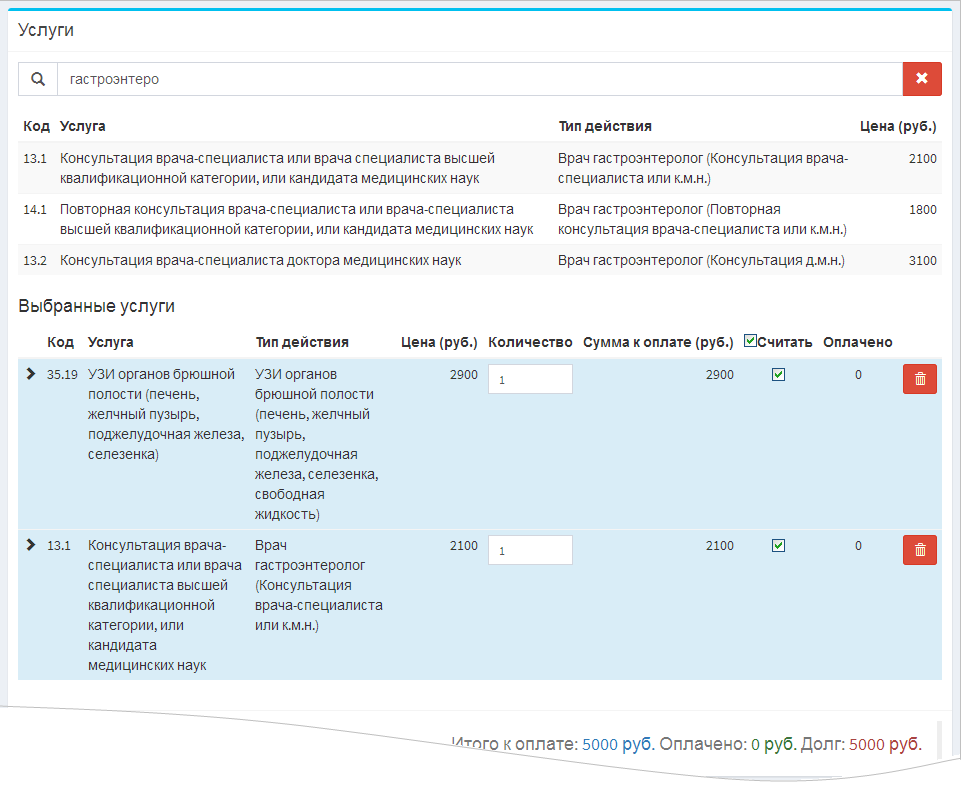
\includegraphics[width = 1\textwidth ,keepaspectratio]{pol_usl}
	\caption{Регистрация услуг в обращении}
	\label{img_pol_usl}
\end{figure}

Для выбранных услуг можно изменить количество в ячейке \dm{Количество} и установить флажок \dm{Считать} для включения стоимость услуг в итоговую сумму в строке <<Итого к оплате>> под таблицей. 

После регистрации требуемого набора услуг необходимо сохранить обращение, после чего распечатать договор и другие платежные документы, нажав кнопку 
\includegraphics[scale=0.6]{print}, выбрав соответствующие пункты из списка и нажав кнопку \btn{Печать}.



\subsection{Обслуживание пациентов (для врача)} \label{pol_ttbl_new}
Если в ЛПУ ведется предварительная запись пациентов на прием по расписанию, то обслуживание пациентов врачом выполняется из раздела \dm{Прием пациентов}. Раздел будет доступен только при наличии у пользователя прав на выполнение данной функции.
Для перехода к обслуживанию пациентов следует на панели управления в верхней части страницы нажать кнопку \dm{Прием пациентов}. Откроется страница управления приемом пациентов (Рисунок \ref{img_ev_obsl}) 

\begin{figure}[ht]\centering
	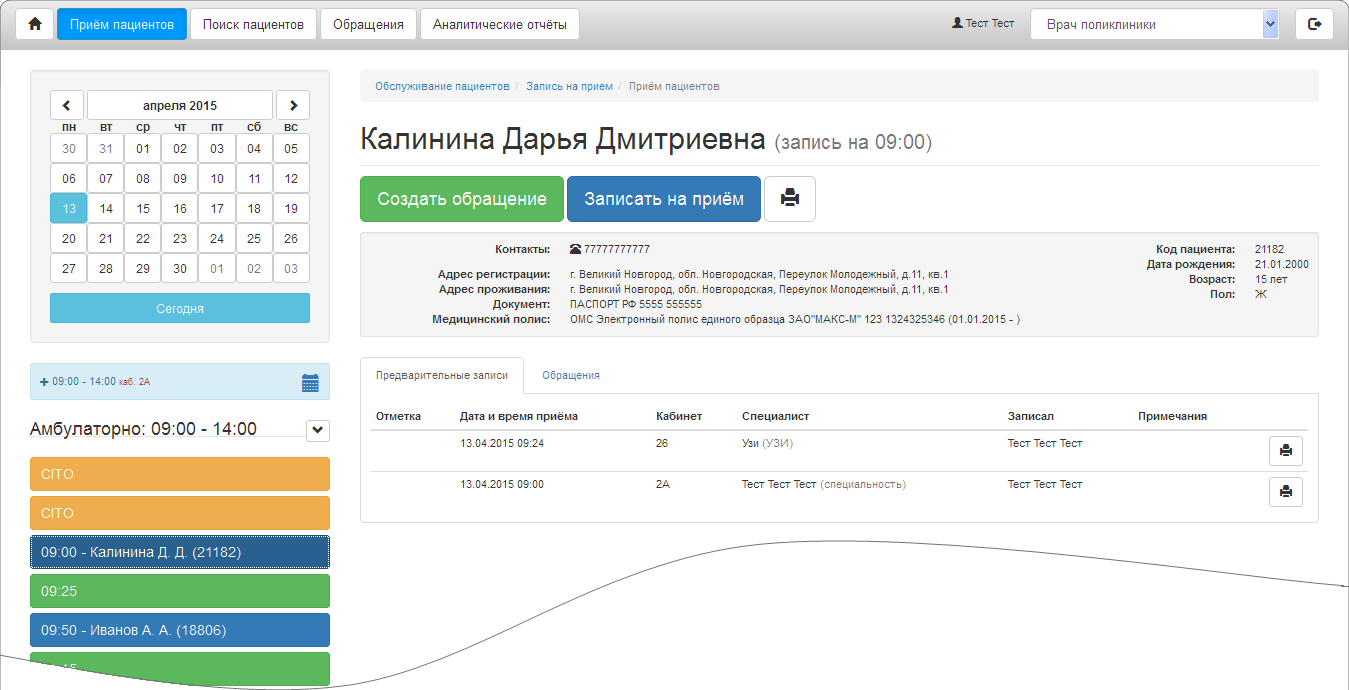
\includegraphics[width = 1\textwidth ,keepaspectratio]{ev_obsl}
	\caption{Страница приема пациентов}
	\label{img_ev_obsl}
\end{figure}

В левой части открывшейся страницы отображаются данные расписания текущего пользователя (под именем которого был осуществлен вход в систему).
В верхней части находится календарь, с помощью которого можно выбрать день для обслуживания или записи пациентов. Для того, чтобы выбрать нужный день месяца, достаточно просто щелкнуть по нему левой кнопкой мыши. Для изменения месяца можно щелкнуть по названию месяца в верхней части календаря и выбрать его из списка. Так же переход к предыдущему или следующему месяцу можно осуществлять с помощью кнопок с изображением стрелок, расположенных слева и справа соответственно от названия месяца в верхней части календаря.

Ниже календаря расположены данные выбранного дня: часы приема и номер кабинета. Нажав на кнопку 
\includegraphics[scale=0.6]{ttbl}, можно просмотреть все свое расписание на отдельной странице.

В левой нижней части страницы расположен список интервалов записи на прием. Интервалы могут иметь следующие цвета:
\begin{itemize}
	\item Зеленый - свободный интервал, на который можно записать пациента.
	\item Синий - интервал, на который записан пациент. Фамилия пациента указана в заголовке интервала.
\end{itemize}

Расписание врача и данные о предварительных записях на прошедшие даты на данной странице просмотреть невозможно.

При нажатии на интевал синего цвета, в правой части страницы появляется информация о пациенте, который записан на данное время:
\begin{itemize}
	\item В верхней части страницы отображаются основные сведения о пациенте: ФИО, контактные данные, адреса, данные документов.
	\item Кнопка \btn{Создать обращение} или \btn{Открыть обращение #....} в левой верхней части данных о пациенте. Если по выбранной предварительной записи обращение еще не создано, то будет отображаться кнопка  \btn{Создать обращение}. Если обращение уже существует -- кнопка \btn{Открыть обращение #....}. 
	\item Кнопка \btn{Записать на прием} в верхней части страницы, при нажатии на которую открывается страница записи пациента к другим специалистам (раздел \ref{pol_predvz}).
	\item Кнопка  \includegraphics[scale=0.6]{prn} в верхней части страницы позволяет распечатать маршрутный лист пациента.
	\item В нижней половине страницы отображаются данные о предварительных записях и обращениях пациента. Данные о предварительных записях доступны на вкладке  \dm{Предварительные записи}. Нажатием на кнопку \includegraphics[scale=0.6]{prn} напротив соответствующей предварительной записи позволяет распечатать маршрутный лист и другие документы по данной предварительной записи. Для просмотра данных об обращениях необходимо перейти на вкладку \dm{Обращения}. Щелчком левой кнопки мыши по обращению можно открыть его для просмотра и, возможно, редактирования.
\end{itemize}  

\subsubsection{Последовательность действий при обслуживании пациента}

При обращении пацинта по предварительной записи, порядок действий врача должен быть следующим:
\begin{enumerate}
	\item В верхней части страницы на панели управления нажать кнопку \btn{Прием пациентов}.
	\item По умолчанию открывается список предварительной записи к текущему врачу на текущую дату. При необходимости, можно изменить дату.
	\item Щелкнуть левой кнопкой мыши по имени пациента в списке предварительной записи. В правой части страницы появятся данные о выбранном пациенте.
	\item Нажать кнопку \btn{Создать обращение} или \btn{Открыть обращение #....} в левой верхней части данных о пациенте. Откроется страница обращения пациента.
	\item Заполнить и сохранить данные текущего обращения пациента (раздел \ref{ev_obr}).
	\item Вернуться на страницу \dm{Прием пациентов} и перейти к обслуживанию следующего пациента.
\end{enumerate}

\subsubsection{Запись пациента на повторный прием} 

Запись пациента на повторный прием удобно выполнять на странице \dm{Прием пациентов}. Для этого нужно:
\begin{enumerate}
	\item Найти пациента в списке предварительной записи и щелкнуть по нему левой кнопкой мыши. Данные пациента появятся в правой части страницы. Если неопсредственно перед этим выполнялось обслуживание пациента, то данное действие уже выполнено.
	\item С помощью календаря в левом верхнем углу страницы перейти на дату, на которую следует записать пациента на повторный прием.
	\item Щелкнуть левой кнопкой мыши по одному из свободных интервалов.
	\item В появившемся диалоговом окне подтвердить запись пациента, нажав кнопку \btn{Записать}. Интервал окрасится в синий цвет и в его названии появится фамилия пациента.
	\item С помощью календаря вернуться в список предварительной записи на текущую дату.
\end{enumerate} 

\subsubsection{Запись пациента к другим специалистам}

Со страницы \dm{Прием пациентов} можно так же записать пациента к другим специалистам. Для этого нужно щелкнуть левой кнопкой мыши по фамилии пациента в списке предварительной записи и после того, как данные пациента появятся в правой части страницы, нажать кнопку \btn{Записать на прием}. В результате, откроется страница предварительной записи на прием пациента к другим специалистам (Рисунок \ref{img_pol_ttbl6}). Работа с эттой страницей подробно описана в разделе \ref{pol_predvz}

\subsection{Работа с обращениями}
\subsubsection{Регистрация обращения (для врача)}

При создании обращения со страницы \dm{Прием пациентов} открывается страница \dm{Создание обращения}. Часть полей заполнена на основе  предварительной записи либо значениями по умолчанию. При регистрации обращения следует проверить и при необходимости скорректировать следующие данные:

\begin{itemize}
	\item \dm{Тип обращения} выбирается из списка значение <<Поликлиника>>. Поле обязательно для заполнения.
	\item \dm{Источник финансирования} – канал оплаты обращения, выбирается из списка. По умолчанию устанавливается первый доступный для пациента истточник финансирования. При регистрации обращения нужно обратить особое внимание на правильность заполнения данного поля. Поле обязательно для заполнения.
	\item \dm{Договор} –- номер договора об оплате выбирается из списка. Состав списка договоров зависит от выбранного источника финансирования. Если в списке доступных договоров присутствует только одна запись, то этот договор устанавливается автоматически. Поле обязательно для заполнения.
	\item \dm{Тип события} -– выбирается из списка. Состав списка изменяется в зависимости от выбранного типа обращения и источника финансирования. Если в отобранном списке присутствует только одна запись, то она устанавливается в поле автоматически. Поле обязательно для заполнения.
	\item \dm{Лечащий врач} –- в поле должна быть указана фамилия текущего врача. Недоступно для редактирования.
	\item \dm{Подразделение} –- отделение поликлиники, в котором обслуживается пациент. Поле обязательно для заполнения.
	\item \dm{Дата начала} –- по умолчанию устанавливается дата предварительной записи. При необходимости дату можно изменить. Поле обязательно для заполнения.
	\item \dm{Время начала} –- по умолчанию устанавливается время предварительной записи. При необходимости время можно изменить. Поле обязательно для заполнения.
	\item \dm{Дата выполнения} –- дата завершения обслуживания по данному обращению. При регистрации обращения не требует заполнения.
	\item \dm{Время выполнения} -– время закрытия обращения. При регистрации обращения не требует заполнения.
	\item \dm{Результат обращения} -- выбирается из списка. При регистрации обращения не требует заполнения.
	\item \dm{Исход заболевания} -- выбирается из списка. При регистрации обращения не требует заполнения.
\end{itemize}

После того как все поля заполнены верно, нужно нажать кнопку \btn{Создать} в правом нижнем углу страницы. Будет осуществлен переход к следующему этапу оформления обращения.




